\documentclass[border=5pt]{standalone}
\usepackage{tikz}
\usepackage{xcolor}
\usetikzlibrary{calc,shadows.blur}

% J12 - Blue rectangular prism (taller)
\begin{document}
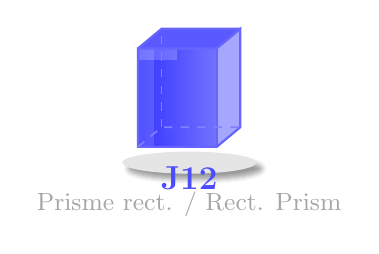
\begin{tikzpicture}

\fill[gray!20,blur shadow={shadow blur steps=5}] (0.65,-0.2) ellipse (0.85 and 0.14);

% Left face
\fill[blue!50] (0,0) -- (0.3,0.25) -- (0.3,1.5) -- (0,1.25) -- cycle;
% Right face
\fill[blue!35] (1.0,0) -- (1.3,0.25) -- (1.3,1.5) -- (1.0,1.25) -- cycle;
% Front face
\fill[left color=blue!80, right color=blue!55] (0,0) -- (1.0,0) -- (1.0,1.25) -- (0,1.25) -- cycle;
% Top face
\fill[blue!65] (0,1.25) -- (1.0,1.25) -- (1.3,1.5) -- (0.3,1.5) -- cycle;

\fill[white,opacity=0.2] (0,1.1) -- (0.5,1.1) -- (0.5,1.25) -- (0,1.25) -- cycle;
\fill[white,opacity=0.15] (0,0) -- (0.2,0) -- (0.2,1.25) -- (0,1.25) -- cycle;

\draw[blue!60, line width=0.8pt] (0,0) -- (1.0,0) -- (1.3,0.25) -- (1.3,1.5) -- (1.0,1.25) -- (0,1.25) -- cycle;
\draw[blue!60, line width=0.8pt] (0,1.25) -- (0.3,1.5) -- (1.3,1.5);
\draw[blue!60, line width=0.8pt] (1.0,0) -- (1.0,1.25);
\draw[blue!50, line width=0.6pt, dashed] (0,0) -- (0.3,0.25) -- (1.3,0.25);
\draw[blue!50, line width=0.6pt, dashed] (0.3,0.25) -- (0.3,1.5);

\node[font=\bfseries\large, text=blue!70] at (0.65,-0.4) {J12};
\node[font=\small, text=gray!70] at (0.65,-0.73) {Prisme rect. / Rect. Prism};
\end{tikzpicture}
\end{document}
